To estimate the MVA output distribution for the top background, we can make use of the 
events in the top-tagged control region weighted by the appropriate function
of the top-tagging efficiency in order to build the prediction of the shape of the
MVA output distribution.

To ensure that this procedure gives an unbiased prediction of the MVA output shape
we show the comparison of the MVA output distribution for the top-tagged 
and the top-vetoed events from the top Monte Carlo simulation. This comparison is shown in
Figure \ref{fig:mva_top}, where we observe agreement within the statistical
uncertainties of the Monte Carlo sample. This is not unexpected since the behavior of
the MVA input observables, all leptonic observables, are not expected to be affected by
whether the event has been b-tagged or not. 

%%%%%%%%%%%%%%%%%%%%%%%%%%%%%%
\begin{figure}[!htbp]
\begin{center}
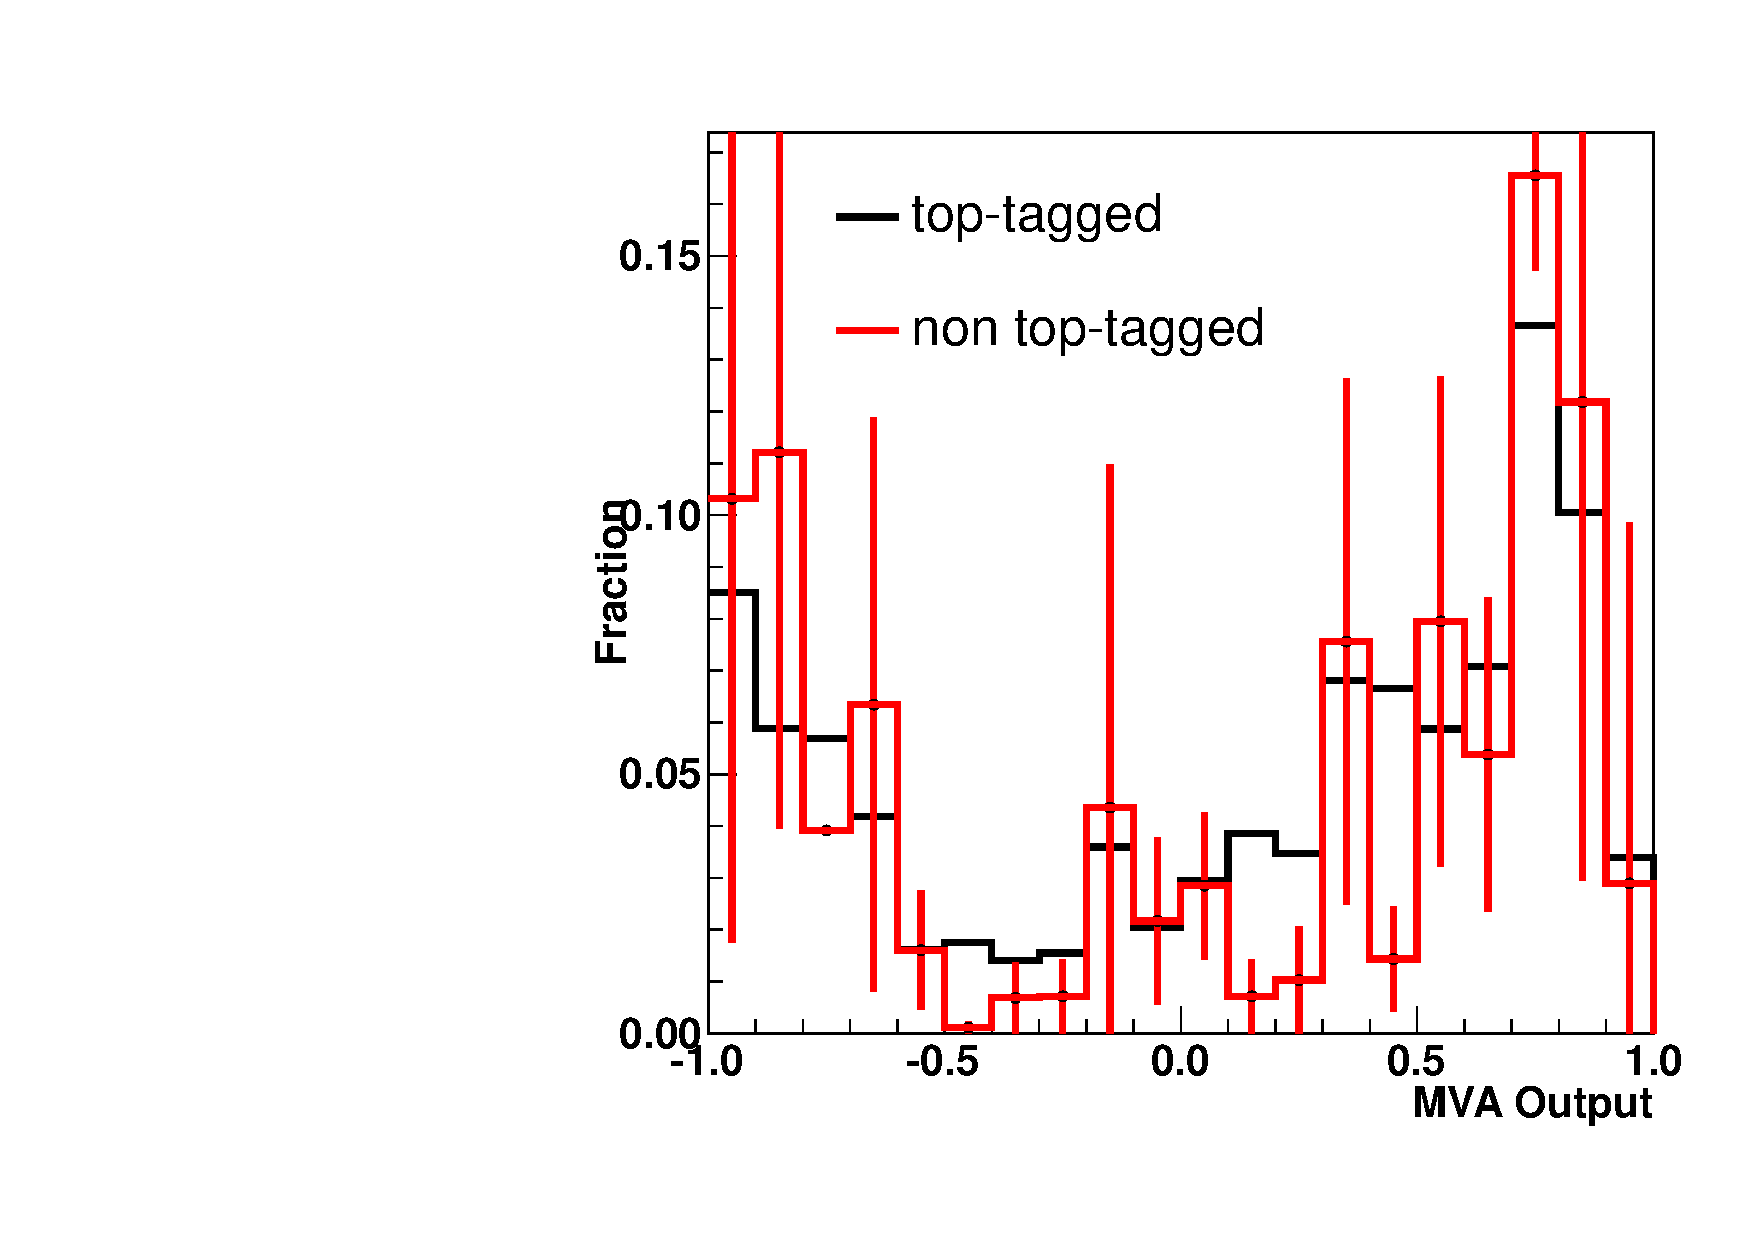
\includegraphics[width=0.7\textwidth]{figures/mva_top.pdf}
\caption{Multivariate output distribution for top-tagged and non top-tagged simulated events.}
\label{fig:mva_top}
\end{center}
\end{figure}
%%%%%%%%%%%%%%%%%%%%%%%%%%%%%%



 
